Motif finding has been studied extensively in the previous years. Numerous algorithms have been made for motif finding and for PMS. These algorithms are categorized as either approximate algorithms or exact algorithms. This section discusses related algorithms that solves the $(l, d)$-planted motif problem including the EMS-GT algorithm.

\section{Approximate Algorithms}
Approximate algorithms, although they are fast, do not guarantee the exact solution all the time. Heuristic algorithms that perform local search such as Gibbs Sampling, Expectation Maximization (EM),  Projections, etc., are previously explored in the literature. Most of these algorithms initially work on a tuple of alignment positions that corresponds to $l$-mers across different string sequences in the dataset. Then they iteratively refine the alignment until a certain criteria has met. MEME \cite{Bailey2006} is a tool for motif finding that implements Expectation Maximization. Other approximate algorithms that use local search are GARP \cite{huo2009combining}, GibbsDNA \cite{lawrence1993detecting} and Random Projection \cite{Buhler2001Tompa, huo2009combining}. WINNOWER \cite{pevzner2000combinatorial} reduces the PMS problem to finding a large clique in a multipartite graph. Instead of looking for the motif directly, the algorithm applies a winnowing technique to remove spurious edges that trims the graph representation making it easier to find the motif. Other approximate algorithms are MULTIPROFILER \cite{Keich01102002},  PatternBranching, ProfileBranching \cite{Price27092003} and CONSENSUS \cite{hertz1999identifying};

% explain one or two approximate then list the rest
\section{Exact Algorithms}
Although they may not be as fast as approximate algorithms, exact algorithms return the correct answer all the time. Furthermore, these exact algorithms can be categorized based on their approach in solving the problem. One approach is to generate a common neighborhood out of all $(m - l + 1)^n$ possible positions representing $l$-mer tuples from all string sequences. This approach is called sample-driven. Another approach is called pattern-driven that checks from $\Sigma^l$ possible $l$-mers which are the motifs. 

Many exact algorithms solve the PMS problem using suffix trees and other related data structures. RISO \cite{Carvalho05ahighly}, RISOTTO \cite{Pisanti06risotto}, SPELLER \cite{Sagot98spellingapproximate} and SMILE are all exact algorithms that use suffix trees. MITRA \cite{eskin2002finding} improves the excessive memory requirement of sample-driven approach by using mismatch tree. Two other algorithms that have some similarity with our algorithm are the Voting algorithm and Bit-based algorithm. Voting algorithm \cite{Chin2005} maintains a hash table that tracks the number the occurrence of every possible $l$-mer and makes sure that every $l$-mer is only counted once in each sequence. An $l$-mer is considered a motif if its total occurrences is equal to the total number of sequences in the dataset.

% Further explain the bit-based algorithm
The Bit-based algorithm \cite{dasari2010efficient} generates the neighborhood of each sequence and intersects it to get the set of motif. It maps every $l$-mer to its corresponding integer value. It uses an array of size $\Sigma^l$ to represent the neighborhood of a sequence and uses the integer representation of an $l$-mer to flag if its a member of the array. It generates the neighborhood of all sequences and merges it using the logical operator AND. The resulting array represents the set of motif.


\subsection{PMS Algorithms Series}
% PMS Series
A series of exact algorithms for the $(l, d)$-planted motif search problem was developed by Rajasekaran et al. The algorithm PMS1 \cite{ExactAlgorithmsPMS} is one of these algorithms. PMS1 solves the problem by enumerating the $d$-neighborhood of all the sequences in the dataset and intersects them, the result is the set of motifs. PMSi and PMSP \cite{Davila2006} are algorithms based on PMS1. PMSi improves the memory space requirement of PMS1 by processing only two sequences at a time. PMSP works by generating all the $d$-neighborhood of each $l$-mer in the first sequence and testing each $d$-neighbor if it exists in the remaining sequences. PMSPrune \cite{pms2007} works the same as PMP but with some improvements. It generates the neighborhood of an $l$-mer using a branch-and-bound approach and implements a pruning strategy to speedup the testing of $l$-mers. Succeeding algorithms like PMS5 \cite{Dinh2011} and PMS6 \cite{Shibdas2014} extend the ideas of PMS1 and PMSPrune. PMS5 generates the common neighborhood of three $l$-mers from different sequences at a time and uses ILP for the pruning process. PMS6 only differs from PMS5 in the way it determines the three $l$-mers.

Quorum PMS is a generalized version of the $(l, d)$-motif search problem. Instead of finding an $l$-mer that exists in all $n$ sequences, it only considers up to $q$. We can see that a qPMS problem is equal to PMS when $q = n$. The qPMS7 \cite{Dinh2012} is one algorithm that solves the qPMS problem. Algorithm qPMS7 is a generalized version of qPMSPrune (quorum version of PMSPrune) combined with the pruning strategy of PMS5 algorithm. 


\subsubsection{PMS8 and qPMS9 Algorithm}
% PMS8 \cite{pms2014} is an algorithm that combines the sample-driven approach and the pattern-driven approach. First, it chooses $k$-tuple $T$ of $l$-mers from $k$ different sequences and it makes sure that all $l$-mers in $T$ has a common neighbor. Each $l$-mer that belongs to the common neighborhood of the tuple $T$ will be checked if it appears in the remaining $n - k$ sequences. The algorithm qPMS9 \cite{pms2015} improves the sample-driven approach of PMS8 by prioritizing $l$-mers that are highly distant from those already in the tuple resulting in a smaller size of common $d$-neighborhood to test and enables the algorithm to process the quorum version of the PMS problem.

The PMS8 \cite{pms2014} algorithm improved its predecessors by using certain pruning conditions in common neighbor generation of a tuple of $l$-mers. The algorithm is composed of 2 parts, the sample driven part and the pattern driven part. The sample driven part generates a tuple of size $k$ from the first $k$ string sequence. The algorithm generates the tuple by choosing an $l$-mer $x$ in sequence $S_i$. After including an $l$-mer in the tuple, the algorithm filters all $l$-mers that has a distance of greater than $2d$ from $x$ in $S_{i+1} ... S_n$ sequences. If the filtering step results to at least one empty row in any sequences in the dataset, it discards $x$ then it proceeds by choosing the next $l$-mer in $S_i$.
If the size of the tuple reached a certain threshold, the algorithm proceeds to the pattern driven part by generating the common neighbors of the $l$-mers in the tuple. 

Given a tuple of $l$-mers $T$, PMS8 uses the consensus total distance of $T$ as a lower bound to check if an $l$-mer $M$ is a common neighbor of the $l$-mers in $T$. The consensus total distance of tuple $T$ is computed by $Cd(T) = \sum_{i=1}^l k - m_i$, where $k$ is the number of $l$-mers in the tuple $T$ and $m_i$ is the maximum frequency of any character in column $i$. PMS8 solves the $(l, d)$-planted motif problem by repeatedly doing the sample driven part and pattern driven part starting from all possible $l$-mers in the first sequence.

The qPMS9 algorithm is an extension of the PMS8 algorithm. In PMS8, everytime it adds an $l$-mer in the tuple $T$, it reorders the remaining string based on the number of alive $l$-mers left in increasing order. This is improved in qPMS9 by changing the criteria into prioritizing strings with the largest minimum additional distance.

% TODO: qPMS9

% --------------------------------------------------------------
\subsection{EMS-GT Algorithm}

The Exact Motif Search - Generate and Test algorithm for the planted motif search problem, first developed by Nabos \cite{nabos2015dissertation}, is composed of main two phases, the Generate phase and the Test phase. The Generate phase takes the first $n'$ number of string sequences in the dataset and generates the set $d$-neighborhood one sequence at a time then intersects it. This accumulates and outputs the set of candidate motifs $\mathcal{C}$ and is composed of $l$-mers that have at least one $d$-neighbor in each of the first $n'$ sequences. The Test phase evaluates each candidate motif $c \in C$ by comparing $c$ if it has at least one $d$-neighbor in each of the remaining $n - n'$ string sequences. \newline

\noindent These phases are formally defined below:
% show the formal definition of EMS-GT algorithm steps
\begin{enumerate} [label={\em (\alph*)}]

	\item {Generate phase} \newline
	This phase operates on the first $n'$ sequences. The intersection of the $d$-neighborhood of each sequence will result to the set of candidate motifs $C$.\newline

	\begin{equation}
		C = \mathcal{N}(S_{1}, d) \cap \mathcal{N}(S_{2}, d) \cap...\cap \mathcal{N}(S_{n'}, d).
	\end{equation} 

	\item {Test phase}\newline
	Each candidate motif in $C$ will be evaluated if it appears in all of the remaining $n - n'$ string sequences. If a candidate motif pass the test, it is then included in the set of motifs $M$. 

\end{enumerate}

% 
The Exact Motif Search - Generate and Test algorithm for the planted motif search problem, first developed by Nabos \cite{nabos2015dissertation}, is composed of main two phases, the Generate phase and the Test phase. The Generate phase takes the first $n'$ number of string sequences in the dataset and generates the set $d$-neighborhood one sequence at a time then intersects it. This accumulates and outputs the set of candidate motifs $\mathcal{C}$ and is composed of $l$-mers that have at least one $d$-neighbor in each of the first $n'$ sequences. The Test phase evaluates each candidate motif $c \in C$ by comparing $c$ if it has at least one $d$-neighbor in each of the remaining $n - n'$ string sequences. \newline

\noindent These phases are formally defined below:
% show the formal definition of EMS-GT algorithm steps
\begin{enumerate} [label={\em (\alph*)}]

	\item {Generate phase} \newline
	This phase operates on the first $n'$ sequences. The intersection of the $d$-neighborhood of each sequence will result to the set of candidate motifs $C$.\newline

	\begin{equation}
		C = \mathcal{N}(S_{1}, d) \cap \mathcal{N}(S_{2}, d) \cap...\cap \mathcal{N}(S_{n'}, d).
	\end{equation} 

	\item {Test phase}\newline
	Each candidate motif in $C$ will be evaluated if it appears in all of the remaining $n - n'$ string sequences. If a candidate motif pass the test, it is then included in the set of motifs $M$. 

\end{enumerate}

% 
The Exact Motif Search - Generate and Test algorithm for the planted motif search problem, first developed by Nabos \cite{nabos2015dissertation}, is composed of main two phases, the Generate phase and the Test phase. The Generate phase takes the first $n'$ number of string sequences in the dataset and generates the set $d$-neighborhood one sequence at a time then intersects it. This accumulates and outputs the set of candidate motifs $\mathcal{C}$ and is composed of $l$-mers that have at least one $d$-neighbor in each of the first $n'$ sequences. The Test phase evaluates each candidate motif $c \in C$ by comparing $c$ if it has at least one $d$-neighbor in each of the remaining $n - n'$ string sequences. \newline

\noindent These phases are formally defined below:
% show the formal definition of EMS-GT algorithm steps
\begin{enumerate} [label={\em (\alph*)}]

	\item {Generate phase} \newline
	This phase operates on the first $n'$ sequences. The intersection of the $d$-neighborhood of each sequence will result to the set of candidate motifs $C$.\newline

	\begin{equation}
		C = \mathcal{N}(S_{1}, d) \cap \mathcal{N}(S_{2}, d) \cap...\cap \mathcal{N}(S_{n'}, d).
	\end{equation} 

	\item {Test phase}\newline
	Each candidate motif in $C$ will be evaluated if it appears in all of the remaining $n - n'$ string sequences. If a candidate motif pass the test, it is then included in the set of motifs $M$. 

\end{enumerate}

% \input{contents/pseudocode/ems-gt}

% \input{contents/pseudocode/recursive-neighborhood-gen}

Data structures and the how an algorithm deals with the data commonly drive the performance of an algorithm. The EMS-GT algorithm uses a compressed bit-flag array for fast candidate motif elimination. Some key techniques that EMS-GT uses are defined in this section.

	\subsubsection{Integer mapping of $l$-mers}
	EMS-GT converts $l$-mers into its corresponding integer values. To achieve this, each character in the $l$-mer is translated using 2 bits (a=00, c=01, g=10, t=11). \newline
		{\small Ex.	\texttt{actg} maps to \texttt{00011110} and has an integer value of 30} 

	\subsubsection{Bit-based set representation and l-mer enumeration} 
	The EMS-GT maintains a $4^l$ array for enumerating all the possible $l$-mer values. The $l$-mer's integer value is used as the index value for the array. It uses the value of 1 if the $l$-mer is a member of the set, else it sets the value to 0.

	\subsubsection{Bit-array compression}
	To efficiently store these $l$-mers and save memory space, EMS-GT implements an approach that compresses the search space array using integer value bit flags. Instead of one $l$-mer per index value, the implementation can flag up to 32 $l$-mers (since we are using 32-bit integers) per index value. The explanation on how the algorithm accesses the bit flag is defined below: \newline

		{\small Ex. \texttt{gacgt} maps to \texttt{1000011011} = 539 in decimal.\newline
			\hspace*{64pt} \emph{bit position} = 539 mod 32 = 27;\newline
			\hspace*{64pt} \emph{array index}  = 539 / 32 = 16;\newline
			\hspace*{64pt} The bit flag for \texttt{gacgt} is in the 27$^{th}$ least significant bit\newline
			\hspace*{64pt} of the integer at array index 16.}

	\input{contents/00_figure/search_space}

	\subsubsection{XOR-based Hamming distance computation}
	The mapping of an $l$-mer to its integer value has an additional advantage in computing for mismatch positions. Applying the boolean operator exclusive-or (XOR) between two integer values will return another integer value that contains nonzero value for mismatch position. Counting this nonzero positions result to the hamming distance value. An example of this computation is shown below: \newline

	{\small Ex.	\texttt{aacgt} maps to \texttt{0000011011} \newline
		\vspace*{2pt}\hspace*{53pt} \underline{\texttt{tacgc} maps to \texttt{1100011001}} \newline
		\hspace*{55pt}	XOR produces \texttt{\uline{11}000000\uline{10}} = 2 mismatches.} \newline
		\hspace*{53pt} (Note, the mismatches are counted per pair)


	\subsubsection{Recursive neighborhood generation}
	The Generate step of the algorithm produces the $d$-neighborhood of a string sequence by generating the $d$-neighborhood of all $l$-mers in that sequence. Our implementation of EMS-GT uses a recursive approach for generating the $d$-neighborhood of an $l$-mer. The recursive generation can be visualized by a tree $\mathcal{T}(x)$ of height $d$ that is generated in depth-first manner. Each node is a tuple of $(w, p)$ where $w$ is an $l$-mer and $p$ corresponds to a position in the $l$-mer $0 \leq p \leq l$. At a given node $(w, p)$ and $p \neq l$, three children nodes are generated where each node is variant of $w$ that has a different character in $p + 1$ position. The root node is $(x, 0)$ and any $l$-mer in nodes at depth $t$ has a hamming distance of $t$ from the $l$-mer $x$. Given this, the expected size of $N(x, d)$ can be computed using the equation: \newline
	\begin{equation}
		|N(x,d)| = \sum_{i=0}^d \binom{l}{i} 3^{i}
	\end{equation}

	\input{contents/00_figure/neighborhood_generation}

	\subsubsection{Block-based optimization for neighborhood generation}
	The way EMS-GT represents the $d$-neighborhood $N_x$ of $l$-mer $x$ opens up a new way to improve the generation of neighborhood. $N_x$ is represented by a compresed $4^l$ bit flags array, where value of 1 corresponds to set membership, 0 if otherwise.  A previous study by Sia \cite{sia2015} improved the runtime performance in generating $N_x$. If $N_x$ is partitioned into blocks of $4^k$ bits each, where $k < l$, each block will conform into ($k$ + 2) bit patterns. By pre-computing these patterns, the algorithm can build the $N_x$ by blocks of bits instead of one bit at a time.

	\input{contents/00_figure/bit-patterns}

	The algorithm divides the $l$-mer $x$ into its $(l - k)$-length prefix $y$ and suffix $z$ of length $k$. With the block patterns of $4^k$ $l$-mers generated, the algorithm recursively generates all possible prefix of $x$. For each prefix $y'$ generated, the algorithm applies the corresponding block pattern in $N_x$ based on $z$ and the remaining number of allowed mutations $d'$, where $d' = d - d_H(y, y')$. Specifically, EMS-GT builds the $\mathcal{N}_S$ using these steps:

	\begin{enumerate}
		\item Initialize $\mathcal{N}_S$ as an array of $4^l$ bits set to zero, and select a value for $k$.

		\item Pre-generate {\em Pattern}( $z$, $d_z$ ) for all $z \in \Sigma^k$ and all $d_z \in \{1,...,k-1\}$ to serve as bit masks for blocks. Note that block patterns for $d_z=0$ (one bit set) and $d_z=k$ (all bits set) will not require bit masks.

		\item For each $l$-mer $x = yz$ in sequence $S$: take each neighbor $y'$ of $y$, find the block in $\mathcal{N}_S$ whose prefix is $y'$, and compute the allowable suffix mismatches $d_z = d - d_H(y,y')$ within this block. Then,

			\begin{enumerate}
				\item if $d_z = 0$, set the bit at position $z$ in the block;
				\item if $d_z \geq k$, set all bits in the block to 1;
				\item otherwise, mask {\em Pattern}( $z$, $d_z$ ) onto the block.
			\end{enumerate}
	\end{enumerate}

	Choosing the optimum value for $k$ is important in this speedup technique. The $k$ value determines the runtime complexity of this technique since $k$ value determines the size of the block patterns. When $k$ value is higher, there are fewer prefix to generate recursively but each block bits setting is large. When $k$ value is lower, block bits setting is small but the algorithm has to recursively generate a larger number of prefix value of $l$-mer $x$. The optimum $k$ value used in the study is 5.

	\input{contents/00_pseudocodes/block-pattern-generation}

	% Elaborate and include results
	% Mention its competitiveness and a bit of introduction on possible areas of improvement 
	EMS-GT with this speedup technique has proven its competitiveness against algorithms qPMSPrune, qPMS7, PMS8 and qPMS9. Previous experimentations showed that EMS-GT with this speedup technique outperforms PMS8 in challenge instances (9, 2), (11, 3), (13, 4), (15, 5) and (17, 6). Compared to qPMS9, the improved EMS-GT is faster on all challenge instances mentioned except (17, 6). This study aims to outperform qPMS9 for challenges up to (17, 6).

	\input{contents/00_figure/sia-bar-results}

% \begin{figure}[b]
	\noindent \hspace*{6pt}{\bf Algorithm 2} \textsc{Generate Neighborhood}
	\begin{algorithmic}[1]
		\label{alg:recursive-nbr-gen}
		\Require DNA sequence $S$, motif length $l$, mismatches $d$
		\Ensure bit-array $\mathcal{N}$ representing $\mathcal{N}(S,d)$ \vspace*{6pt}
		% \For{$i \leftarrow$ 1 to $4^{l}$}
		\State $\mathcal{N}[i] \leftarrow 0,\ \ \forall i < 4^{l}$ 
		% \EndFor
		\For{each $l$-mer $x$ in $S$}
			\State \textsc{AddNeighbors}($x$, 0, $d$) \hspace*{9pt}\Comment{recursive procedure}
		\EndFor
		\State \Comment{make $d$ changes in $l$-mer $x$, from position $s$ onward}
		\Procedure{AddNeighbors}{$x$, $s$, $d$}
			\For{$i \leftarrow s$ to $l$}
				\State $\Sigma \leftarrow$ \{\texttt{a}, \texttt{g}, \texttt{c}, \texttt{t}\} $- x_{i}$ \hspace*{6pt}\Comment{$i^{th}$ character in $x$}
				\For{$j \leftarrow 1$ to $|\Sigma|$}
					\State $neighbor \leftarrow\ ${\em\small concatenate}$(x_{1...i-1},\Sigma_{j},x_{i+1...l})$
					\State $\mathcal{N}[neighbor] \leftarrow 1$
					\If{$d > 1$ and $i < l$}
						\State \textsc{AddNeighbors}($neighbor$, $i+1$, $d-1$)
					\EndIf
				\EndFor
			\EndFor
		\EndProcedure
		\State\Return $\mathcal{N}$
	\end{algorithmic}
\end{figure}

Data structures and the how an algorithm deals with the data commonly drive the performance of an algorithm. The EMS-GT algorithm uses a compressed bit-flag array for fast candidate motif elimination. Some key techniques that EMS-GT uses are defined in this section.

	\subsubsection{Integer mapping of $l$-mers}
	EMS-GT converts $l$-mers into its corresponding integer values. To achieve this, each character in the $l$-mer is translated using 2 bits (a=00, c=01, g=10, t=11). \newline
		{\small Ex.	\texttt{actg} maps to \texttt{00011110} and has an integer value of 30} 

	\subsubsection{Bit-based set representation and l-mer enumeration} 
	The EMS-GT maintains a $4^l$ array for enumerating all the possible $l$-mer values. The $l$-mer's integer value is used as the index value for the array. It uses the value of 1 if the $l$-mer is a member of the set, else it sets the value to 0.

	\subsubsection{Bit-array compression}
	To efficiently store these $l$-mers and save memory space, EMS-GT implements an approach that compresses the search space array using integer value bit flags. Instead of one $l$-mer per index value, the implementation can flag up to 32 $l$-mers (since we are using 32-bit integers) per index value. The explanation on how the algorithm accesses the bit flag is defined below: \newline

		{\small Ex. \texttt{gacgt} maps to \texttt{1000011011} = 539 in decimal.\newline
			\hspace*{64pt} \emph{bit position} = 539 mod 32 = 27;\newline
			\hspace*{64pt} \emph{array index}  = 539 / 32 = 16;\newline
			\hspace*{64pt} The bit flag for \texttt{gacgt} is in the 27$^{th}$ least significant bit\newline
			\hspace*{64pt} of the integer at array index 16.}

	\begin{figure}[h]
	\centering
	\label{fig:search_space}
	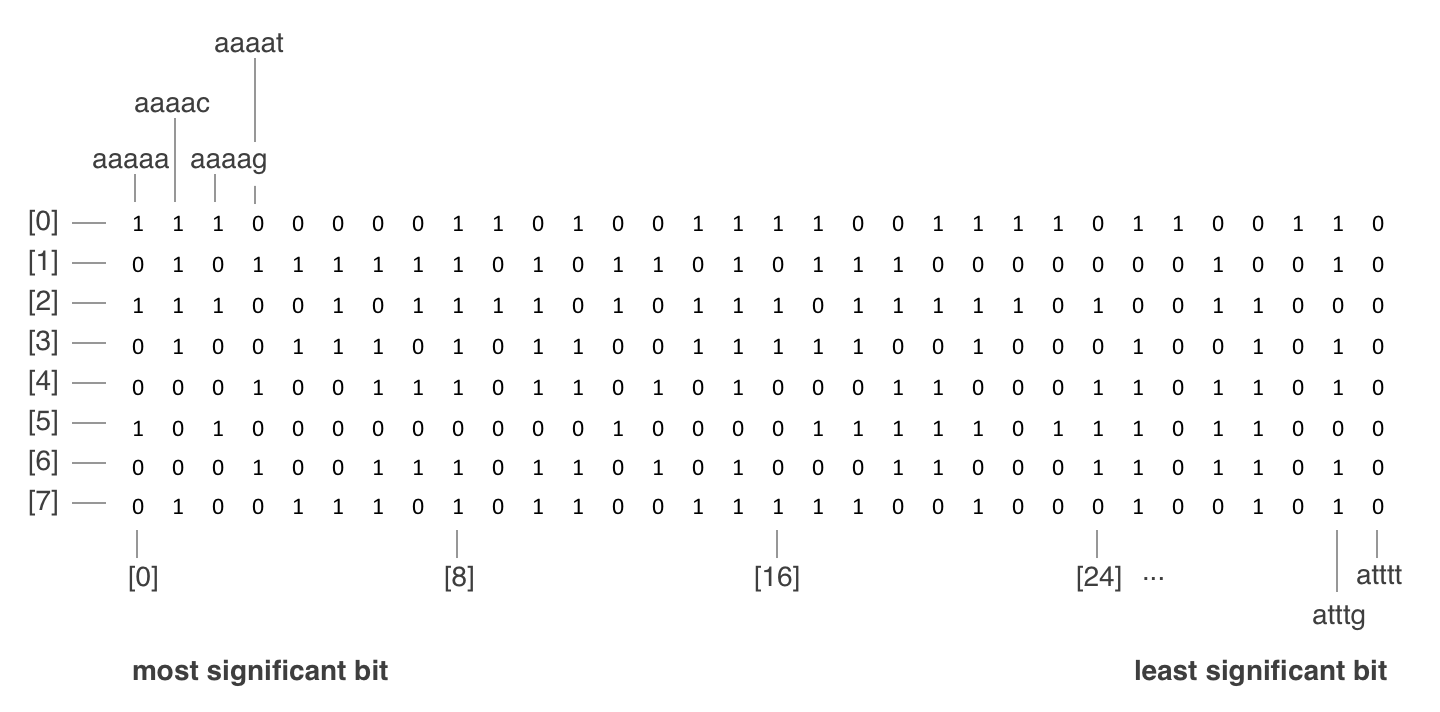
\includegraphics[width=5in]{contents/00_images/search_space}\vspace*{5pt}
	\caption{First 8 rows of the $4^{5}$ search space with random flag values.}
\end{figure}

	\subsubsection{XOR-based Hamming distance computation}
	The mapping of an $l$-mer to its integer value has an additional advantage in computing for mismatch positions. Applying the boolean operator exclusive-or (XOR) between two integer values will return another integer value that contains nonzero value for mismatch position. Counting this nonzero positions result to the hamming distance value. An example of this computation is shown below: \newline

	{\small Ex.	\texttt{aacgt} maps to \texttt{0000011011} \newline
		\vspace*{2pt}\hspace*{53pt} \underline{\texttt{tacgc} maps to \texttt{1100011001}} \newline
		\hspace*{55pt}	XOR produces \texttt{\uline{11}000000\uline{10}} = 2 mismatches.} \newline
		\hspace*{53pt} (Note, the mismatches are counted per pair)


	\subsubsection{Recursive neighborhood generation}
	The Generate step of the algorithm produces the $d$-neighborhood of a string sequence by generating the $d$-neighborhood of all $l$-mers in that sequence. Our implementation of EMS-GT uses a recursive approach for generating the $d$-neighborhood of an $l$-mer. The recursive generation can be visualized by a tree $\mathcal{T}(x)$ of height $d$ that is generated in depth-first manner. Each node is a tuple of $(w, p)$ where $w$ is an $l$-mer and $p$ corresponds to a position in the $l$-mer $0 \leq p \leq l$. At a given node $(w, p)$ and $p \neq l$, three children nodes are generated where each node is variant of $w$ that has a different character in $p + 1$ position. The root node is $(x, 0)$ and any $l$-mer in nodes at depth $t$ has a hamming distance of $t$ from the $l$-mer $x$. Given this, the expected size of $N(x, d)$ can be computed using the equation: \newline
	\begin{equation}
		|N(x,d)| = \sum_{i=0}^d \binom{l}{i} 3^{i}
	\end{equation}

	\begin{figure}[h]
	\centering
	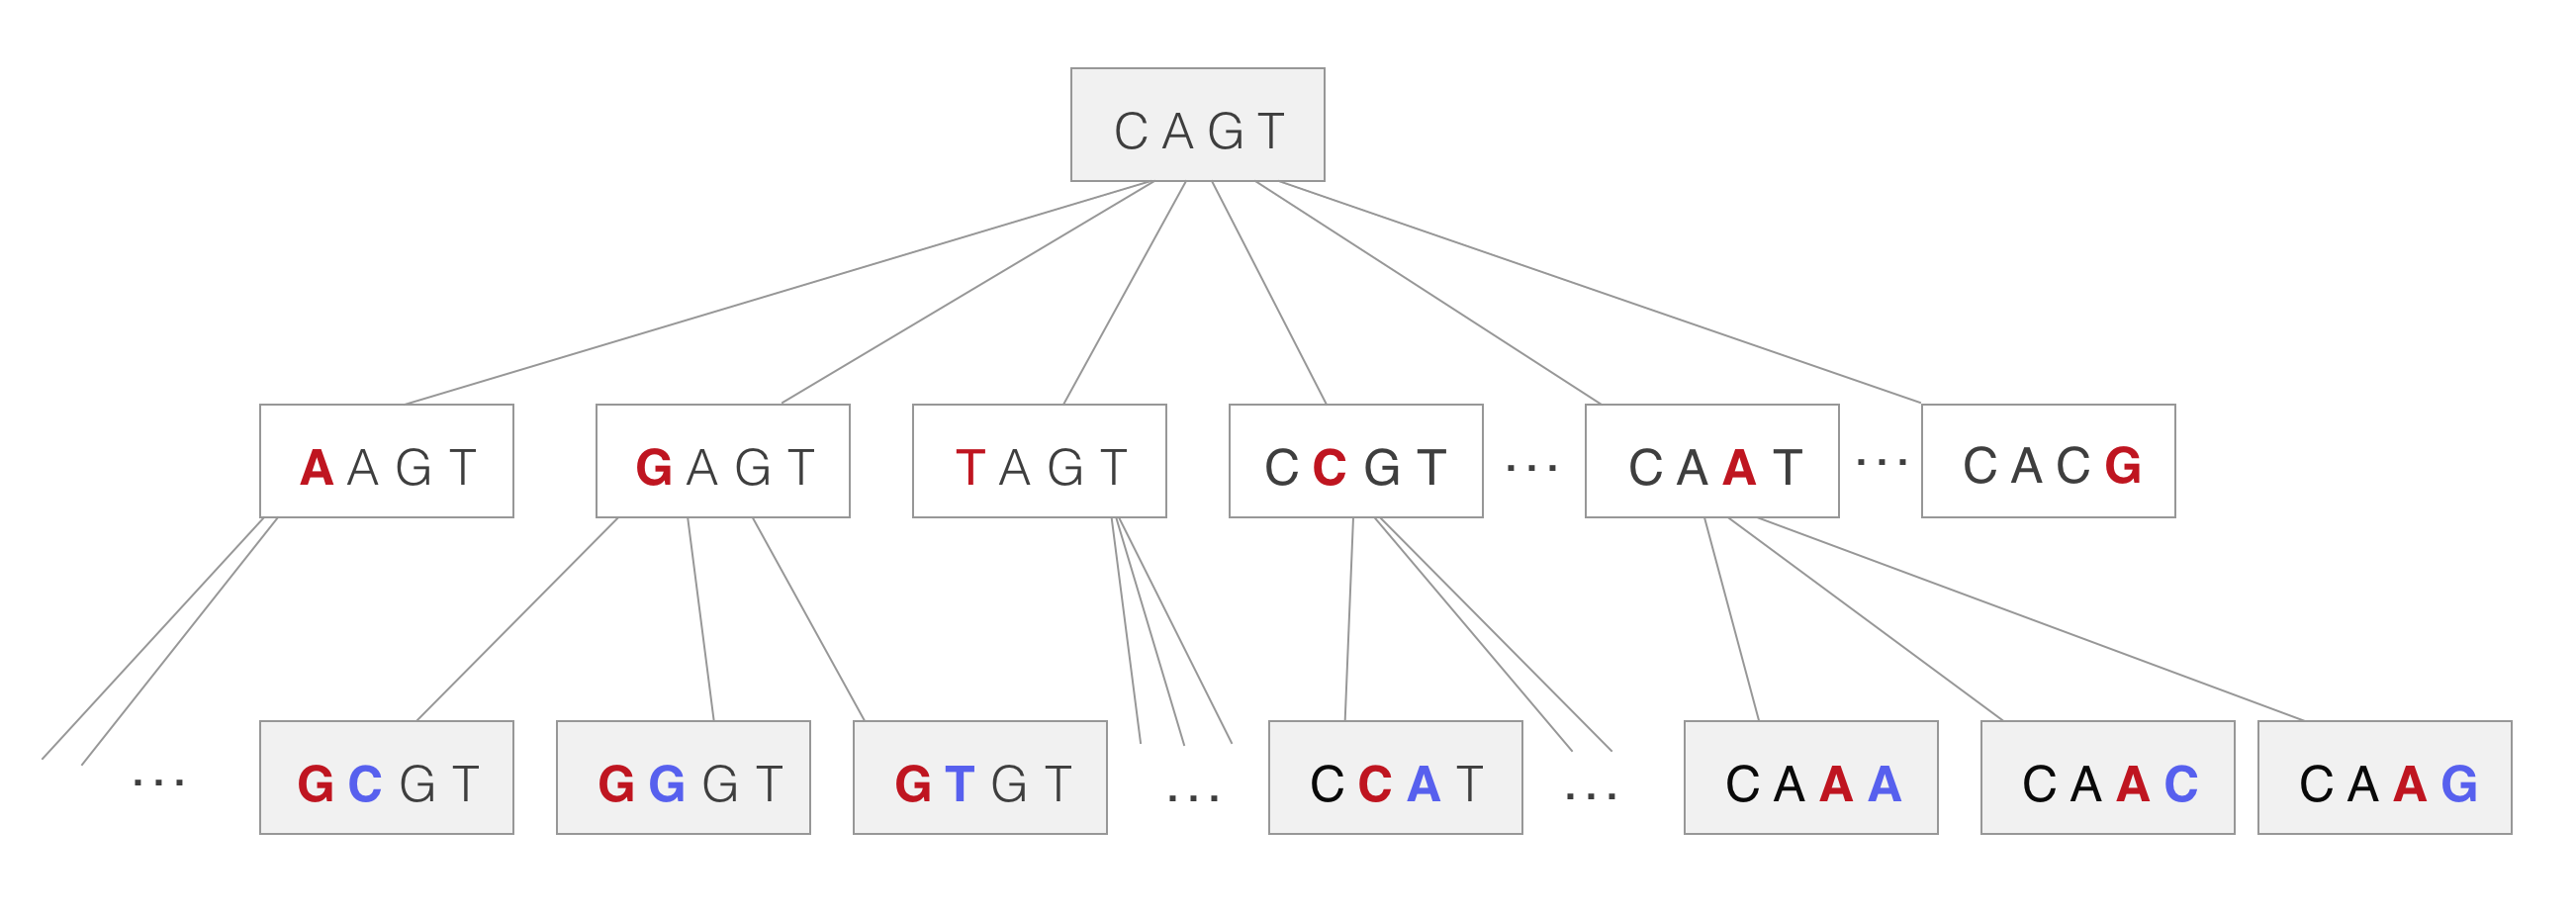
\includegraphics[width=5in]{contents/00_images/neighborhood-generation}\vspace*{5pt}
	\caption{Recursively generating the neighborhood of $l$-mer CACGT with $d = 2$}
	\label{fig:neighborhood-generation}
\end{figure}

	\subsubsection{Block-based optimization for neighborhood generation}
	The way EMS-GT represents the $d$-neighborhood $N_x$ of $l$-mer $x$ opens up a new way to improve the generation of neighborhood. $N_x$ is represented by a compresed $4^l$ bit flags array, where value of 1 corresponds to set membership, 0 if otherwise.  A previous study by Sia \cite{sia2015} improved the runtime performance in generating $N_x$. If $N_x$ is partitioned into blocks of $4^k$ bits each, where $k < l$, each block will conform into ($k$ + 2) bit patterns. By pre-computing these patterns, the algorithm can build the $N_x$ by blocks of bits instead of one bit at a time.

	\begin{figure}[h]
	\centering
	
\includegraphics[width=2.5in]{contents/00_images/0-1}\vspace*{5pt}
	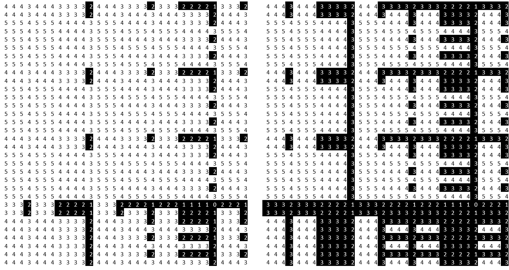
\includegraphics[width=2.5in]{contents/00_images/2-3}\vspace*{5pt}
	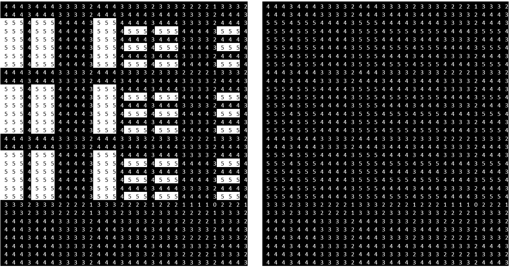
\includegraphics[width=2.5in]{contents/00_images/4-5}
	
	\caption{Bit patterns followed by blocks of size $4^{5}=32\times32$ in the bit-based representation of $\mathcal{N}(\texttt{acgtacgtacgt},5)$. Black signifies a 1. There are $(5+2)=7$ possible patterns---the empty pattern (all 0s) is not shown. Images from \cite{sia2015}}
	\label{fig:bit_patterns}
\end{figure}

	The algorithm divides the $l$-mer $x$ into its $(l - k)$-length prefix $y$ and suffix $z$ of length $k$. With the block patterns of $4^k$ $l$-mers generated, the algorithm recursively generates all possible prefix of $x$. For each prefix $y'$ generated, the algorithm applies the corresponding block pattern in $N_x$ based on $z$ and the remaining number of allowed mutations $d'$, where $d' = d - d_H(y, y')$. Specifically, EMS-GT builds the $\mathcal{N}_S$ using these steps:

	\begin{enumerate}
		\item Initialize $\mathcal{N}_S$ as an array of $4^l$ bits set to zero, and select a value for $k$.

		\item Pre-generate {\em Pattern}( $z$, $d_z$ ) for all $z \in \Sigma^k$ and all $d_z \in \{1,...,k-1\}$ to serve as bit masks for blocks. Note that block patterns for $d_z=0$ (one bit set) and $d_z=k$ (all bits set) will not require bit masks.

		\item For each $l$-mer $x = yz$ in sequence $S$: take each neighbor $y'$ of $y$, find the block in $\mathcal{N}_S$ whose prefix is $y'$, and compute the allowable suffix mismatches $d_z = d - d_H(y,y')$ within this block. Then,

			\begin{enumerate}
				\item if $d_z = 0$, set the bit at position $z$ in the block;
				\item if $d_z \geq k$, set all bits in the block to 1;
				\item otherwise, mask {\em Pattern}( $z$, $d_z$ ) onto the block.
			\end{enumerate}
	\end{enumerate}

	Choosing the optimum value for $k$ is important in this speedup technique. The $k$ value determines the runtime complexity of this technique since $k$ value determines the size of the block patterns. When $k$ value is higher, there are fewer prefix to generate recursively but each block bits setting is large. When $k$ value is lower, block bits setting is small but the algorithm has to recursively generate a larger number of prefix value of $l$-mer $x$. The optimum $k$ value used in the study is 5.

	
% {\setstretch{1.0} % Algorithm 4.1. Block Pattern Generation
\begin{figure}[h]
	\noindent \hspace*{6pt}{\bf Algorithm 2.1}
	\textsc{Block Pattern Generation}\small
	\begin{algorithmic}[1]\label{alg:block-pattern-gen}
		\Require block degree $k$
		\Ensure 3D bit-array $\mathcal{P}$ containing all possible non-trivial block patterns \vspace*{6pt}

		\State $\mathcal{P}[\ ][\ ][\ ] \leftarrow \{\}$ \hspace*{90pt}
		\Comment{retrieve a pattern $P$ as $\mathcal{P}[z][d - d_{y'}]$ }

		\For {$z \leftarrow 0$ to $4^k$}
		\For {$j \leftarrow 1$ to $k-1$}
		\For {$z' \leftarrow 0$ to $4^k$}
		\If{$dH(z,z') \leq j$} 
			\State $\mathcal{P}[z][j][z'] \leftarrow 1$
		\Else
			\State $\mathcal{P}[z][j][z'] \leftarrow 0$
		\EndIf\EndFor\EndFor\EndFor
		\State\Return $\mathcal{P}$
		\end{algorithmic}
\end{figure}



	% Elaborate and include results
	% Mention its competitiveness and a bit of introduction on possible areas of improvement 
	EMS-GT with this speedup technique has proven its competitiveness against algorithms qPMSPrune, qPMS7, PMS8 and qPMS9. Previous experimentations showed that EMS-GT with this speedup technique outperforms PMS8 in challenge instances (9, 2), (11, 3), (13, 4), (15, 5) and (17, 6). Compared to qPMS9, the improved EMS-GT is faster on all challenge instances mentioned except (17, 6). This study aims to outperform qPMS9 for challenges up to (17, 6).

	
\begin{figure}[ht]\label{fig:results2}
	\centering
	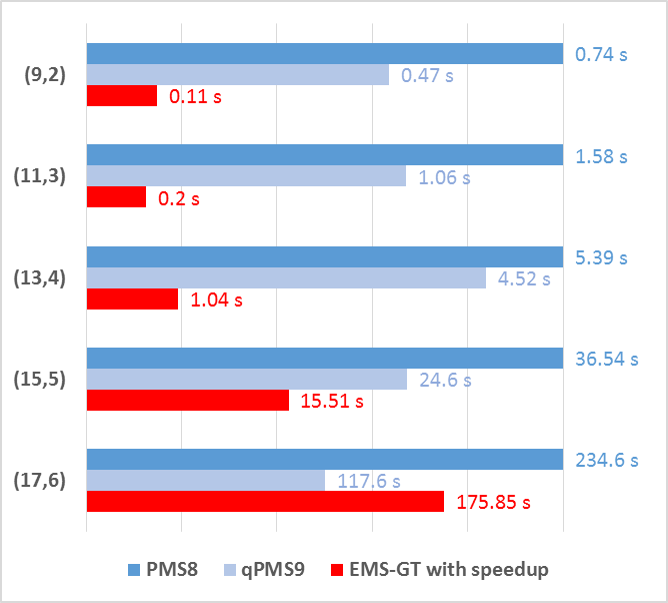
\includegraphics[width=4.0in]{contents/00_images/emsgt-with-speedup-vs-PMS,qPMS9}
	\caption{Improved EMS-GT's performance vs. PMS8 (baseline) and qPMS9. Images from \cite{sia2015}}
	\label{fig:sia-bar-results}
\end{figure}

% \begin{figure}[b]
	\noindent \hspace*{6pt}{\bf Algorithm 2} \textsc{Generate Neighborhood}
	\begin{algorithmic}[1]
		\label{alg:recursive-nbr-gen}
		\Require DNA sequence $S$, motif length $l$, mismatches $d$
		\Ensure bit-array $\mathcal{N}$ representing $\mathcal{N}(S,d)$ \vspace*{6pt}
		% \For{$i \leftarrow$ 1 to $4^{l}$}
		\State $\mathcal{N}[i] \leftarrow 0,\ \ \forall i < 4^{l}$ 
		% \EndFor
		\For{each $l$-mer $x$ in $S$}
			\State \textsc{AddNeighbors}($x$, 0, $d$) \hspace*{9pt}\Comment{recursive procedure}
		\EndFor
		\State \Comment{make $d$ changes in $l$-mer $x$, from position $s$ onward}
		\Procedure{AddNeighbors}{$x$, $s$, $d$}
			\For{$i \leftarrow s$ to $l$}
				\State $\Sigma \leftarrow$ \{\texttt{a}, \texttt{g}, \texttt{c}, \texttt{t}\} $- x_{i}$ \hspace*{6pt}\Comment{$i^{th}$ character in $x$}
				\For{$j \leftarrow 1$ to $|\Sigma|$}
					\State $neighbor \leftarrow\ ${\em\small concatenate}$(x_{1...i-1},\Sigma_{j},x_{i+1...l})$
					\State $\mathcal{N}[neighbor] \leftarrow 1$
					\If{$d > 1$ and $i < l$}
						\State \textsc{AddNeighbors}($neighbor$, $i+1$, $d-1$)
					\EndIf
				\EndFor
			\EndFor
		\EndProcedure
		\State\Return $\mathcal{N}$
	\end{algorithmic}
\end{figure}

Data structures and the how an algorithm deals with the data commonly drive the performance of an algorithm. The EMS-GT algorithm uses a compressed bit-flag array for fast candidate motif elimination. Some key techniques that EMS-GT uses are defined in this section.

	\subsubsection{Integer mapping of $l$-mers}
	EMS-GT converts $l$-mers into its corresponding integer values. To achieve this, each character in the $l$-mer is translated using 2 bits (a=00, c=01, g=10, t=11). \newline
		{\small Ex.	\texttt{actg} maps to \texttt{00011110} and has an integer value of 30} 

	\subsubsection{Bit-based set representation and l-mer enumeration} 
	The EMS-GT maintains a $4^l$ array for enumerating all the possible $l$-mer values. The $l$-mer's integer value is used as the index value for the array. It uses the value of 1 if the $l$-mer is a member of the set, else it sets the value to 0.

	\subsubsection{Bit-array compression}
	To efficiently store these $l$-mers and save memory space, EMS-GT implements an approach that compresses the search space array using integer value bit flags. Instead of one $l$-mer per index value, the implementation can flag up to 32 $l$-mers (since we are using 32-bit integers) per index value. The explanation on how the algorithm accesses the bit flag is defined below: \newline

		{\small Ex. \texttt{gacgt} maps to \texttt{1000011011} = 539 in decimal.\newline
			\hspace*{64pt} \emph{bit position} = 539 mod 32 = 27;\newline
			\hspace*{64pt} \emph{array index}  = 539 / 32 = 16;\newline
			\hspace*{64pt} The bit flag for \texttt{gacgt} is in the 27$^{th}$ least significant bit\newline
			\hspace*{64pt} of the integer at array index 16.}

	\begin{figure}[h]
	\centering
	\label{fig:search_space}
	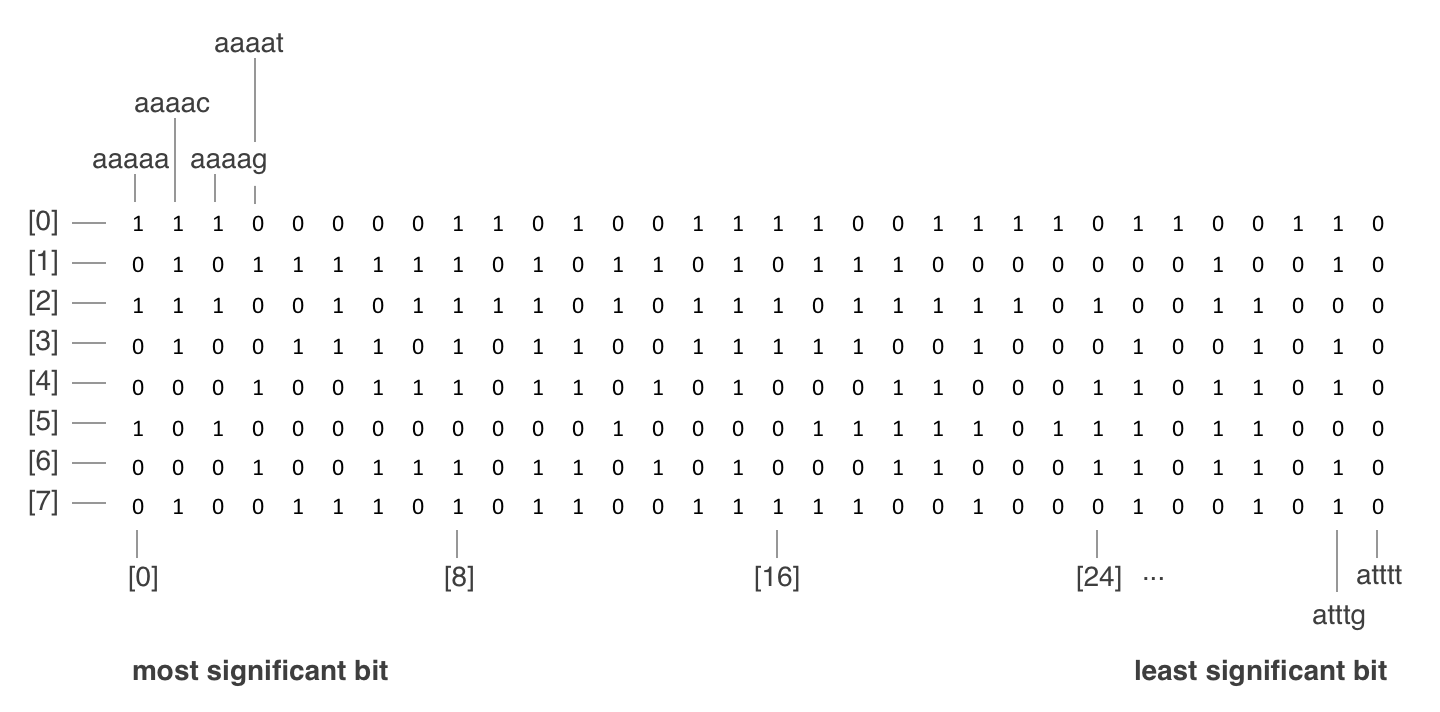
\includegraphics[width=5in]{contents/00_images/search_space}\vspace*{5pt}
	\caption{First 8 rows of the $4^{5}$ search space with random flag values.}
\end{figure}

	\subsubsection{XOR-based Hamming distance computation}
	The mapping of an $l$-mer to its integer value has an additional advantage in computing for mismatch positions. Applying the boolean operator exclusive-or (XOR) between two integer values will return another integer value that contains nonzero value for mismatch position. Counting this nonzero positions result to the hamming distance value. An example of this computation is shown below: \newline

	{\small Ex.	\texttt{aacgt} maps to \texttt{0000011011} \newline
		\vspace*{2pt}\hspace*{53pt} \underline{\texttt{tacgc} maps to \texttt{1100011001}} \newline
		\hspace*{55pt}	XOR produces \texttt{\uline{11}000000\uline{10}} = 2 mismatches.} \newline
		\hspace*{53pt} (Note, the mismatches are counted per pair)


	\subsubsection{Recursive neighborhood generation}
	The Generate step of the algorithm produces the $d$-neighborhood of a string sequence by generating the $d$-neighborhood of all $l$-mers in that sequence. Our implementation of EMS-GT uses a recursive approach for generating the $d$-neighborhood of an $l$-mer. The recursive generation can be visualized by a tree $\mathcal{T}(x)$ of height $d$ that is generated in depth-first manner. Each node is a tuple of $(w, p)$ where $w$ is an $l$-mer and $p$ corresponds to a position in the $l$-mer $0 \leq p \leq l$. At a given node $(w, p)$ and $p \neq l$, three children nodes are generated where each node is variant of $w$ that has a different character in $p + 1$ position. The root node is $(x, 0)$ and any $l$-mer in nodes at depth $t$ has a hamming distance of $t$ from the $l$-mer $x$. Given this, the expected size of $N(x, d)$ can be computed using the equation: \newline
	\begin{equation}
		|N(x,d)| = \sum_{i=0}^d \binom{l}{i} 3^{i}
	\end{equation}

	\begin{figure}[h]
	\centering
	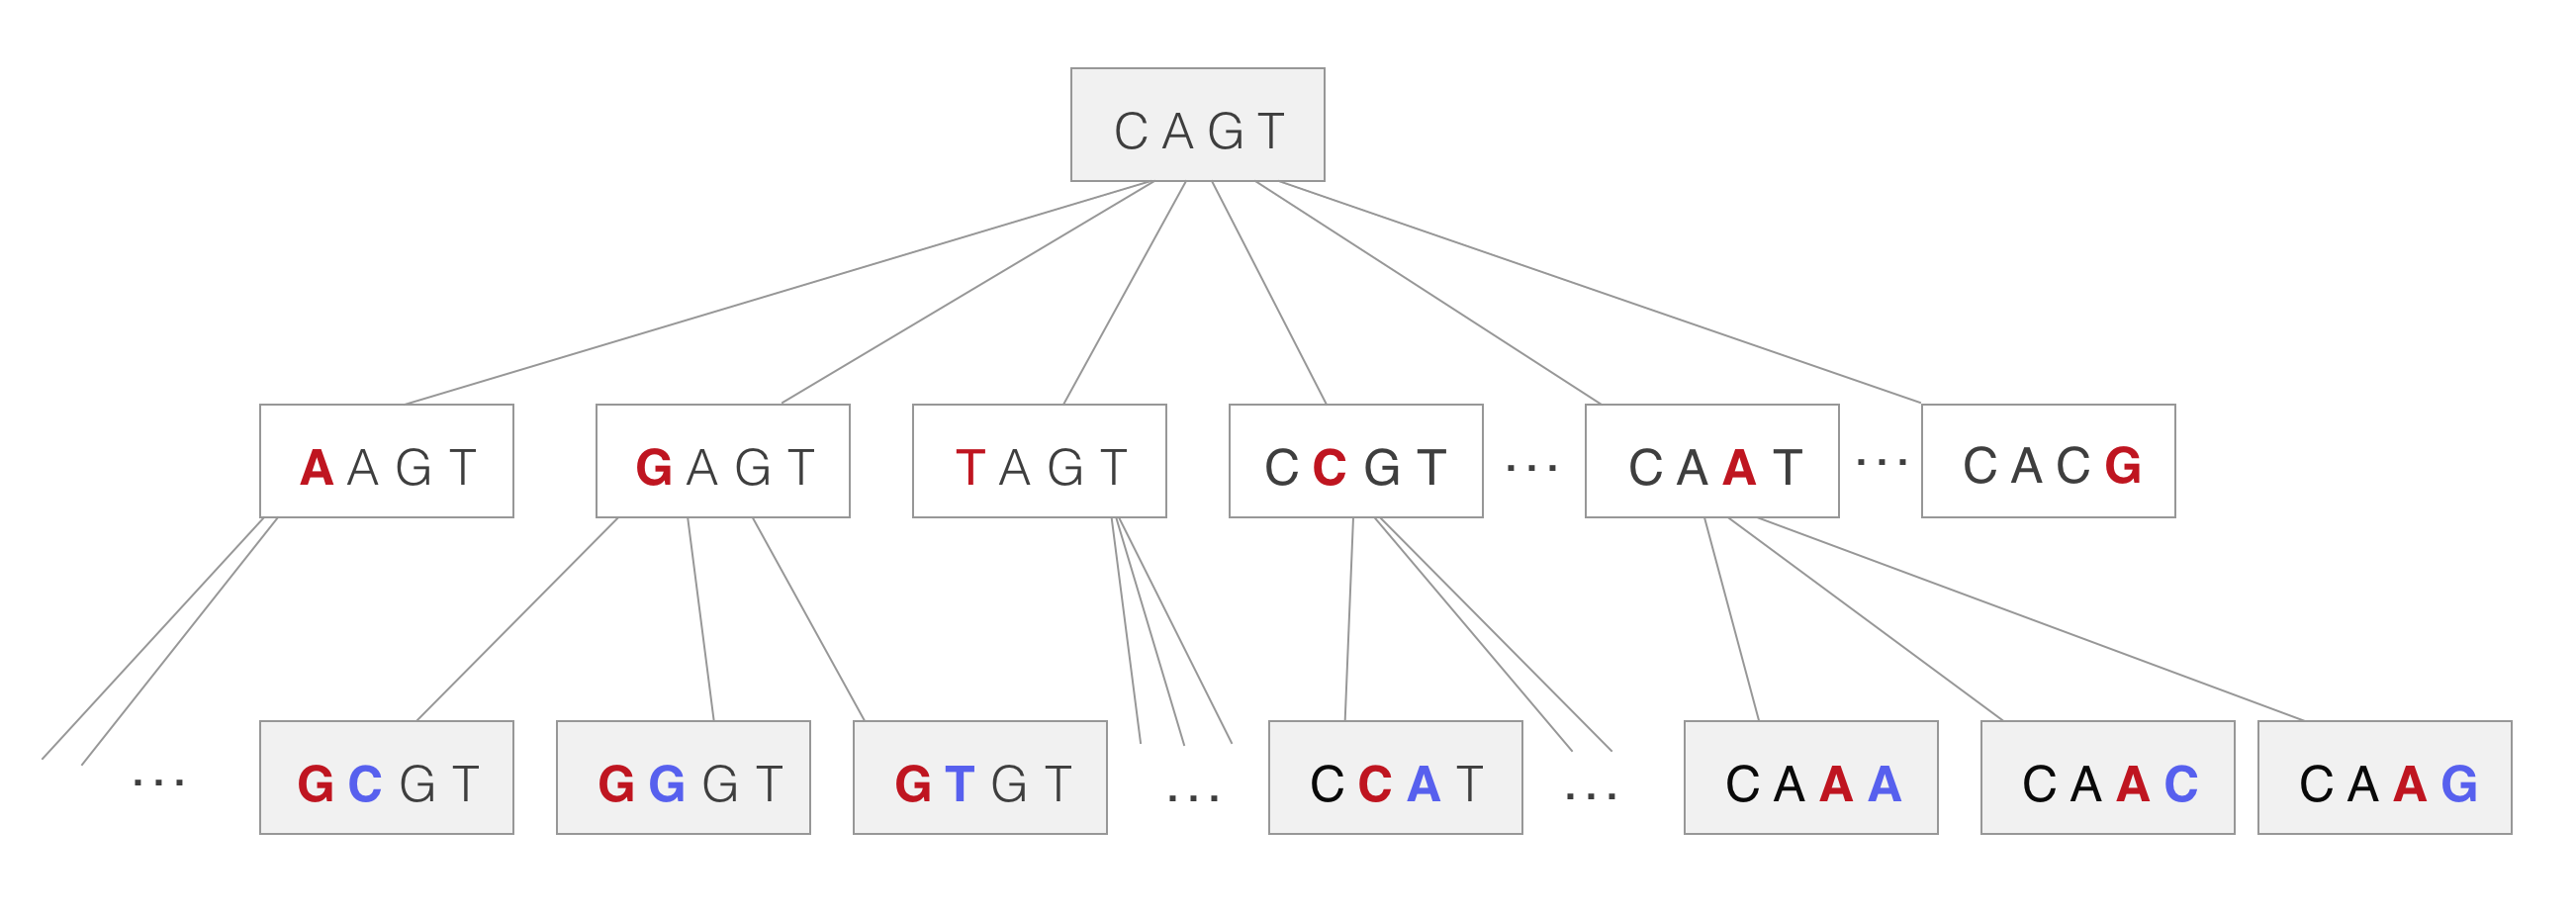
\includegraphics[width=5in]{contents/00_images/neighborhood-generation}\vspace*{5pt}
	\caption{Recursively generating the neighborhood of $l$-mer CACGT with $d = 2$}
	\label{fig:neighborhood-generation}
\end{figure}

	\subsubsection{Block-based optimization for neighborhood generation}
	The way EMS-GT represents the $d$-neighborhood $N_x$ of $l$-mer $x$ opens up a new way to improve the generation of neighborhood. $N_x$ is represented by a compresed $4^l$ bit flags array, where value of 1 corresponds to set membership, 0 if otherwise.  A previous study by Sia \cite{sia2015} improved the runtime performance in generating $N_x$. If $N_x$ is partitioned into blocks of $4^k$ bits each, where $k < l$, each block will conform into ($k$ + 2) bit patterns. By pre-computing these patterns, the algorithm can build the $N_x$ by blocks of bits instead of one bit at a time.

	\begin{figure}[h]
	\centering
	
\includegraphics[width=2.5in]{contents/00_images/0-1}\vspace*{5pt}
	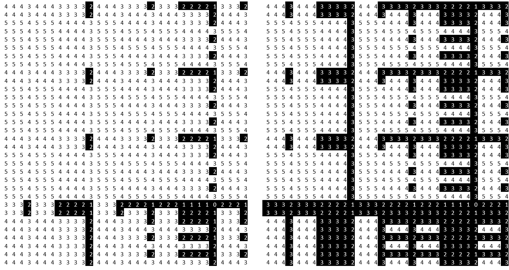
\includegraphics[width=2.5in]{contents/00_images/2-3}\vspace*{5pt}
	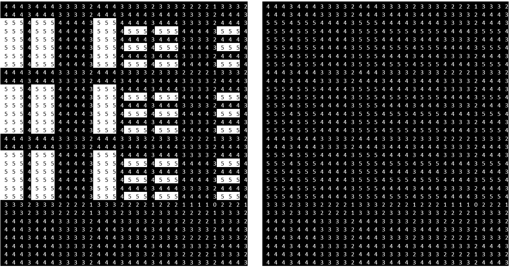
\includegraphics[width=2.5in]{contents/00_images/4-5}
	
	\caption{Bit patterns followed by blocks of size $4^{5}=32\times32$ in the bit-based representation of $\mathcal{N}(\texttt{acgtacgtacgt},5)$. Black signifies a 1. There are $(5+2)=7$ possible patterns---the empty pattern (all 0s) is not shown. Images from \cite{sia2015}}
	\label{fig:bit_patterns}
\end{figure}

	The algorithm divides the $l$-mer $x$ into its $(l - k)$-length prefix $y$ and suffix $z$ of length $k$. With the block patterns of $4^k$ $l$-mers generated, the algorithm recursively generates all possible prefix of $x$. For each prefix $y'$ generated, the algorithm applies the corresponding block pattern in $N_x$ based on $z$ and the remaining number of allowed mutations $d'$, where $d' = d - d_H(y, y')$. Specifically, EMS-GT builds the $\mathcal{N}_S$ using these steps:

	\begin{enumerate}
		\item Initialize $\mathcal{N}_S$ as an array of $4^l$ bits set to zero, and select a value for $k$.

		\item Pre-generate {\em Pattern}( $z$, $d_z$ ) for all $z \in \Sigma^k$ and all $d_z \in \{1,...,k-1\}$ to serve as bit masks for blocks. Note that block patterns for $d_z=0$ (one bit set) and $d_z=k$ (all bits set) will not require bit masks.

		\item For each $l$-mer $x = yz$ in sequence $S$: take each neighbor $y'$ of $y$, find the block in $\mathcal{N}_S$ whose prefix is $y'$, and compute the allowable suffix mismatches $d_z = d - d_H(y,y')$ within this block. Then,

			\begin{enumerate}
				\item if $d_z = 0$, set the bit at position $z$ in the block;
				\item if $d_z \geq k$, set all bits in the block to 1;
				\item otherwise, mask {\em Pattern}( $z$, $d_z$ ) onto the block.
			\end{enumerate}
	\end{enumerate}

	Choosing the optimum value for $k$ is important in this speedup technique. The $k$ value determines the runtime complexity of this technique since $k$ value determines the size of the block patterns. When $k$ value is higher, there are fewer prefix to generate recursively but each block bits setting is large. When $k$ value is lower, block bits setting is small but the algorithm has to recursively generate a larger number of prefix value of $l$-mer $x$. The optimum $k$ value used in the study is 5.

	
% {\setstretch{1.0} % Algorithm 4.1. Block Pattern Generation
\begin{figure}[h]
	\noindent \hspace*{6pt}{\bf Algorithm 2.1}
	\textsc{Block Pattern Generation}\small
	\begin{algorithmic}[1]\label{alg:block-pattern-gen}
		\Require block degree $k$
		\Ensure 3D bit-array $\mathcal{P}$ containing all possible non-trivial block patterns \vspace*{6pt}

		\State $\mathcal{P}[\ ][\ ][\ ] \leftarrow \{\}$ \hspace*{90pt}
		\Comment{retrieve a pattern $P$ as $\mathcal{P}[z][d - d_{y'}]$ }

		\For {$z \leftarrow 0$ to $4^k$}
		\For {$j \leftarrow 1$ to $k-1$}
		\For {$z' \leftarrow 0$ to $4^k$}
		\If{$dH(z,z') \leq j$} 
			\State $\mathcal{P}[z][j][z'] \leftarrow 1$
		\Else
			\State $\mathcal{P}[z][j][z'] \leftarrow 0$
		\EndIf\EndFor\EndFor\EndFor
		\State\Return $\mathcal{P}$
		\end{algorithmic}
\end{figure}



	% Elaborate and include results
	% Mention its competitiveness and a bit of introduction on possible areas of improvement 
	EMS-GT with this speedup technique has proven its competitiveness against algorithms qPMSPrune, qPMS7, PMS8 and qPMS9. Previous experimentations showed that EMS-GT with this speedup technique outperforms PMS8 in challenge instances (9, 2), (11, 3), (13, 4), (15, 5) and (17, 6). Compared to qPMS9, the improved EMS-GT is faster on all challenge instances mentioned except (17, 6). This study aims to outperform qPMS9 for challenges up to (17, 6).

	
\begin{figure}[ht]\label{fig:results2}
	\centering
	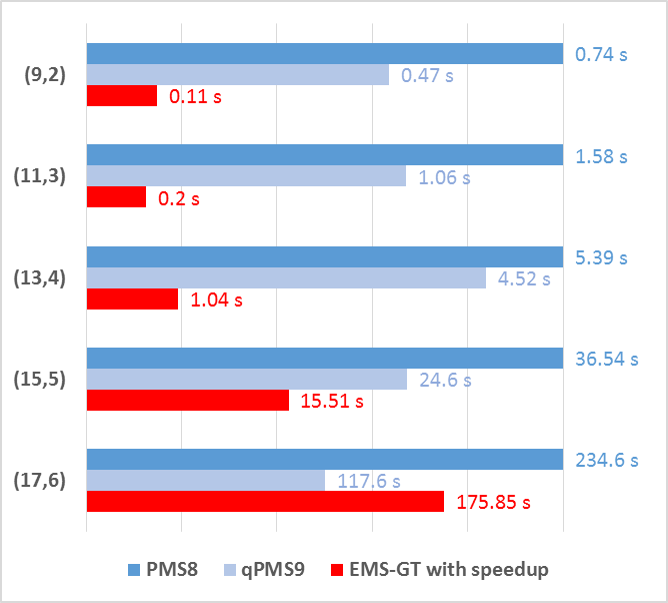
\includegraphics[width=4.0in]{contents/00_images/emsgt-with-speedup-vs-PMS,qPMS9}
	\caption{Improved EMS-GT's performance vs. PMS8 (baseline) and qPMS9. Images from \cite{sia2015}}
	\label{fig:sia-bar-results}
\end{figure}


